\documentclass[english,hidelinks,xetex, 11 pt, class=report,crop=false]{standalone}
\input{../../preamb_cyrillic}
\input{../uk}




\begin{document}
\pagestyle{fancy}
\fancyhead{}
\fancyhead[C]{
\footnotesize Переклад з англійської на українську за допомогою ChatGPT. Можуть з'являтися дивні слова та речення.
}

\section{Додавання}

\subsubsection{Порядок дій}
Цей метод ґрунтується на системі розрядів, де ми почергово обчислюємо суму одиниць, десятків, сотень і так далі.
\begin{center}
	\parbox{0.3\linewidth}{
		\eks[1]{
			\begin{figure}
				\centering
				\includegraphics[]{rekfig/plus1}
			\end{figure}
		}
	}\qquad
	\parbox{0.3\linewidth}{
		\eks[2]{
			\begin{figure}
				\centering
				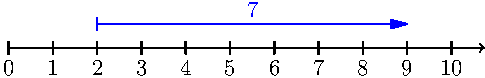
\includegraphics[]{rekfig/plus2}
			\end{figure}
		}
	}\\[12pt]
	\parbox{0.3\linewidth}{
		\eks[3]{
			\begin{figure}
				\centering
				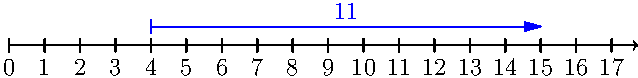
\includegraphics[]{rekfig/plus3}
			\end{figure}
	}}\qquad
	\parbox{0.3\linewidth}{
		\eks[4]{
			\begin{figure}
				\centering
				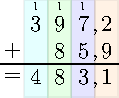
\includegraphics[]{rekfig/plus4}
			\end{figure}
	}}
\end{center}
\fork{Приклад 1}{
	\begin{figure}
		\centering
		\subfloat[]{\includegraphics{rekfig/plus1a}}\qquad
		\subfloat[]{\includegraphics{rekfig/plus1b}}\qquad
		\subfloat[]{\includegraphics{rekfig/plus1c}}
	\end{figure}
	
	\begin{enumerate}[label=\alph*)]
		\item Ми додаємо одиниці: $ 4+2=6 $
		\item Ми додаємо десятки: $ 3+1=4 $
		\item Ми додаємо сотні: $ 2+6=8 $
	\end{enumerate}
} \newpage
\fork{Приклад 2}{
	\begin{figure}
		\centering
		\subfloat[]{\includegraphics{rekfig/plus2a}}\qquad
		\subfloat[]{\includegraphics{rekfig/plus2b}}\qquad
		\subfloat[]{\includegraphics{rekfig/plus2c}}
	\end{figure}
	
	\begin{enumerate}[label=\alph*)]
		\item Ми додаємо одиниці: $ 3+6=9 $
		\item Ми додаємо десятки: $ {7+8=15} $. Оскільки 10 десятків дорівнює 100, ми додаємо 1 на місце сотень і записуємо залишених 5 десятків на місце десятків.
		\item Ми додаємо сотні: $ 1+2=3 $.
	\end{enumerate}
} \vsk

\end{document}